%%%%%%%%%%%%%%%%%%%%%%%%%%%%%%%%%%%%%%%%%%%%%%%%%%%%%%%%
%%%%%%%%%%%%%%%%%%%%%%%%%%%%%%%%%%%%%%%%%%%%%%%%%%%%%%%%
%%%%%%%%%%%%%%%%%%%%%%%%%%%%%%%%%%%%%%%%%%%%%%%%%%%%%%%%
\chapter{Probability Distributions}
\label{dist}

% Place these distributions first as they are simple and keep the interesting ones together on the next page
\begin{figure}
  \centering
  \savebox{\largestimage}{
    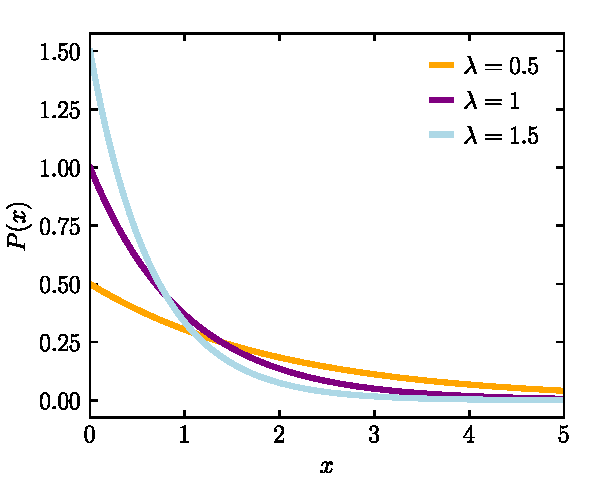
\includegraphics[width=0.47\textwidth]{figures/stats/dist/exp_pdf}
  }% Store largest image in a box

  \begin{subfigure}[b]{0.48\textwidth}\centering
    \raisebox{\dimexpr.5\ht\largestimage-.5\height}{% Adjust vertical height of smaller image
      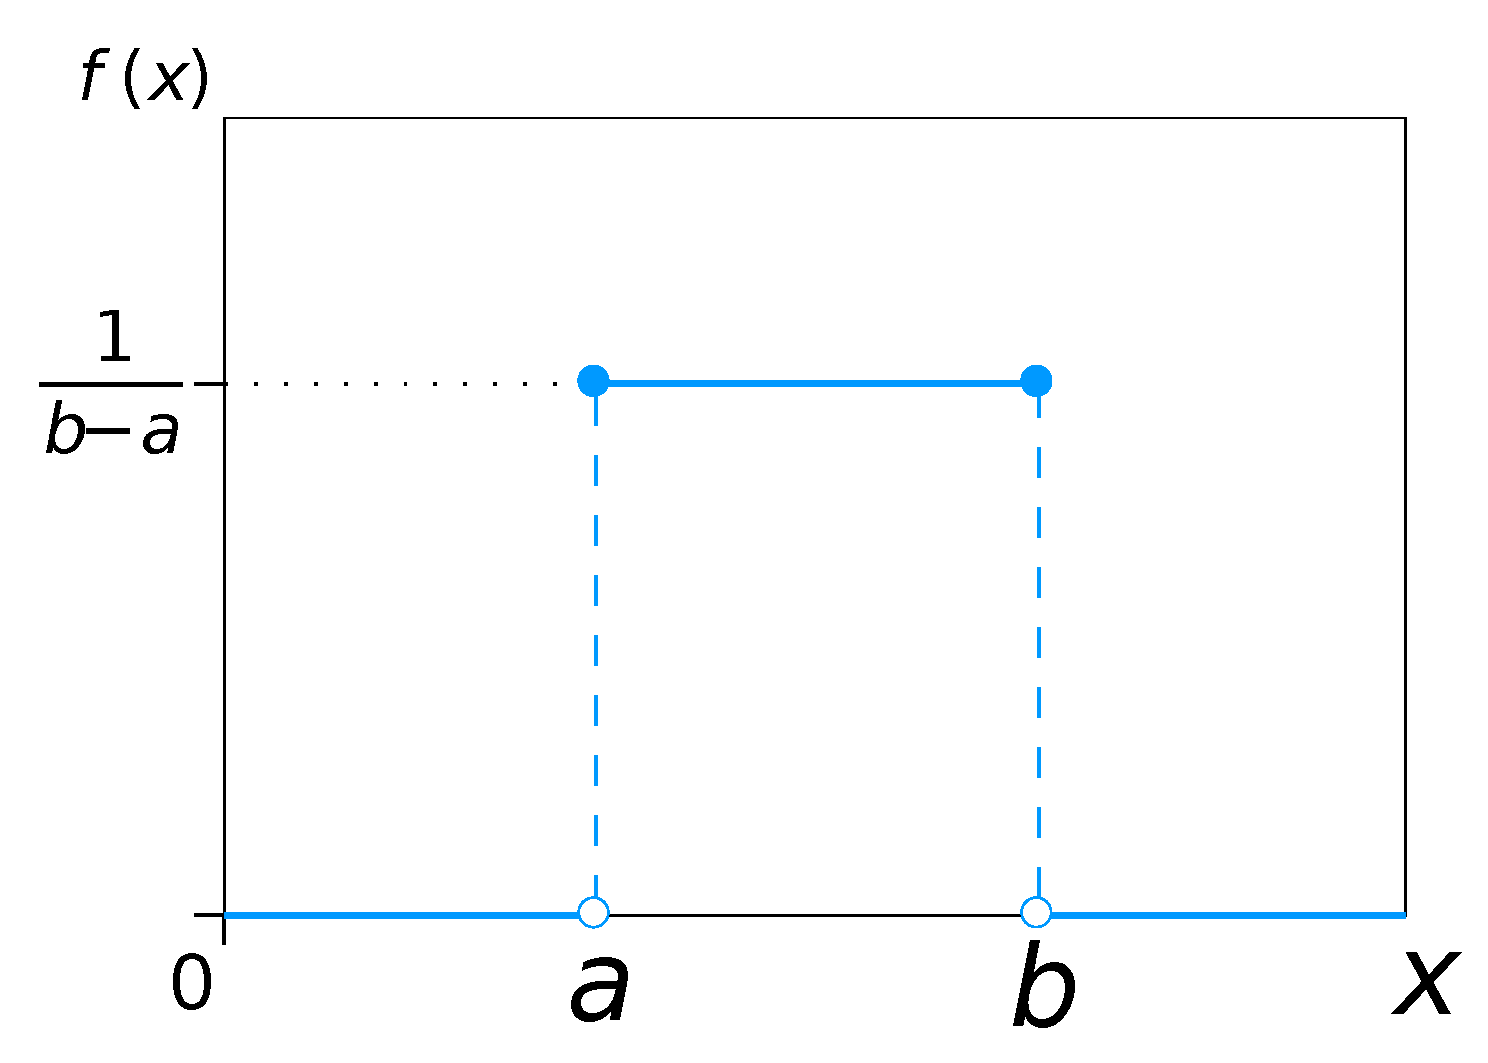
\includegraphics[width=\textwidth]{figures/stats/dist/uniform_pdf}}
  \caption{Uniform Distribution PDF}
  \label{fig:dist:uniform}
  \end{subfigure}
  ~
  \begin{subfigure}[b]{\wd\largestimage}\centering
    \usebox{\largestimage}
  \caption{Exponential Distribution PDF}
  \label{fig:dist:exp}
  \end{subfigure}
\caption{
Uniform and exponential distribution PDFs,
by \href{https://en.wikipedia.org/wiki/File:Uniform_Distribution_PDF_SVG.svg}{AnonMoos}
and \href{https://en.wikipedia.org/wiki/File:Exponential_probability_density.svg}{AkanoToE}.
\label{fig:dist:uniform_exp}
}
\end{figure}

\begin{figure}
  \centering
  \savebox{\largestimage}{
    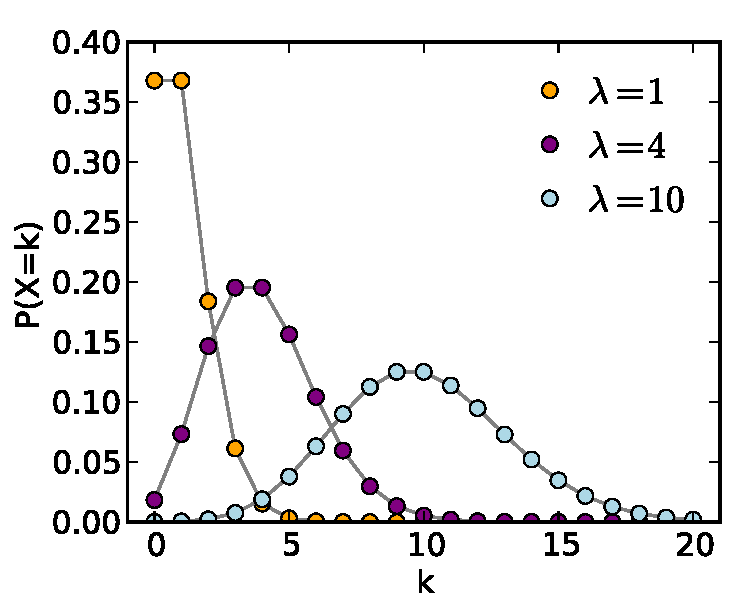
\includegraphics[width=0.47\textwidth]{figures/stats/dist/poisson_pmf}
  }% Store largest image in a box

  \begin{subfigure}[b]{\wd\largestimage}\centering
    \raisebox{\dimexpr.5\ht\largestimage-.5\height}{% Adjust vertical height of smaller image
      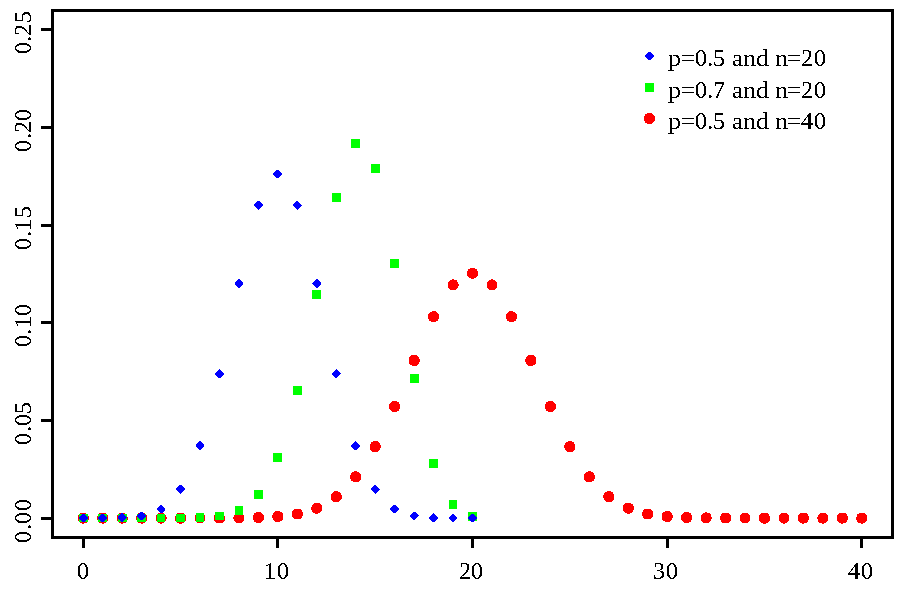
\includegraphics[width=\textwidth]{figures/stats/dist/binomial_pmf}}
  \caption{Binomial Distribution PMF}
  \label{fig:dist:binomial}
  \end{subfigure}
  ~
  \begin{subfigure}[b]{0.48\textwidth}\centering
    \usebox{\largestimage}
  \caption{Poisson Distribution PMF}
  \label{fig:dist:poisson}
  \end{subfigure}
\caption{
Binomial and Poisson distribution PMFs,
by \href{https://en.wikipedia.org/wiki/File:Binomial_distribution_pmf.svg}{Tayste}
and \href{https://en.wikipedia.org/wiki/File:Poisson_pmf.svg}{Skbkekas}.
Both plots have $k$ on the $x$-axis and $P$ on the $y$-axis, and curves for various $n$ and $p$, or $\lambda$.
\label{fig:dist:binomial_poisson}
}
\end{figure}

\begin{figure}
  \centering
  \savebox{\largestimage}{
    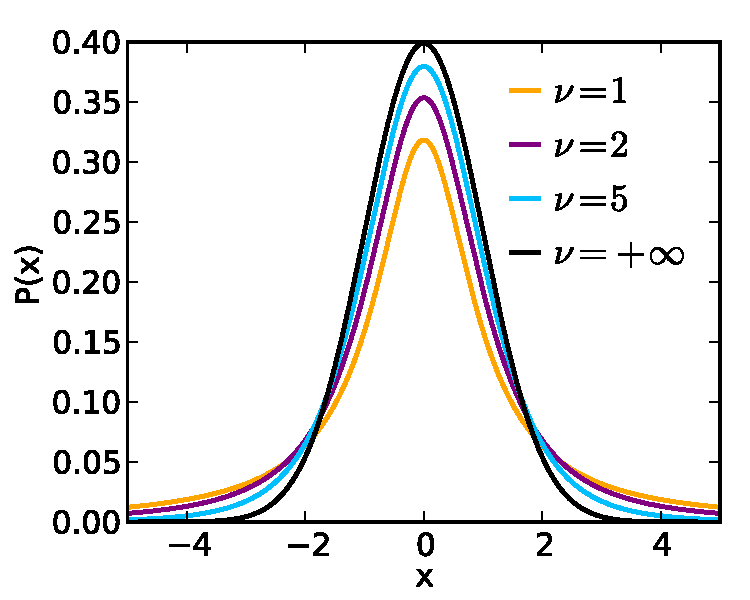
\includegraphics[width=0.47\textwidth]{figures/stats/dist/student_t_pdf}
  }% Store largest image in a box

  \begin{subfigure}[b]{0.48\textwidth}\centering
    \raisebox{\dimexpr.5\ht\largestimage-.5\height}{% Adjust vertical height of smaller image
      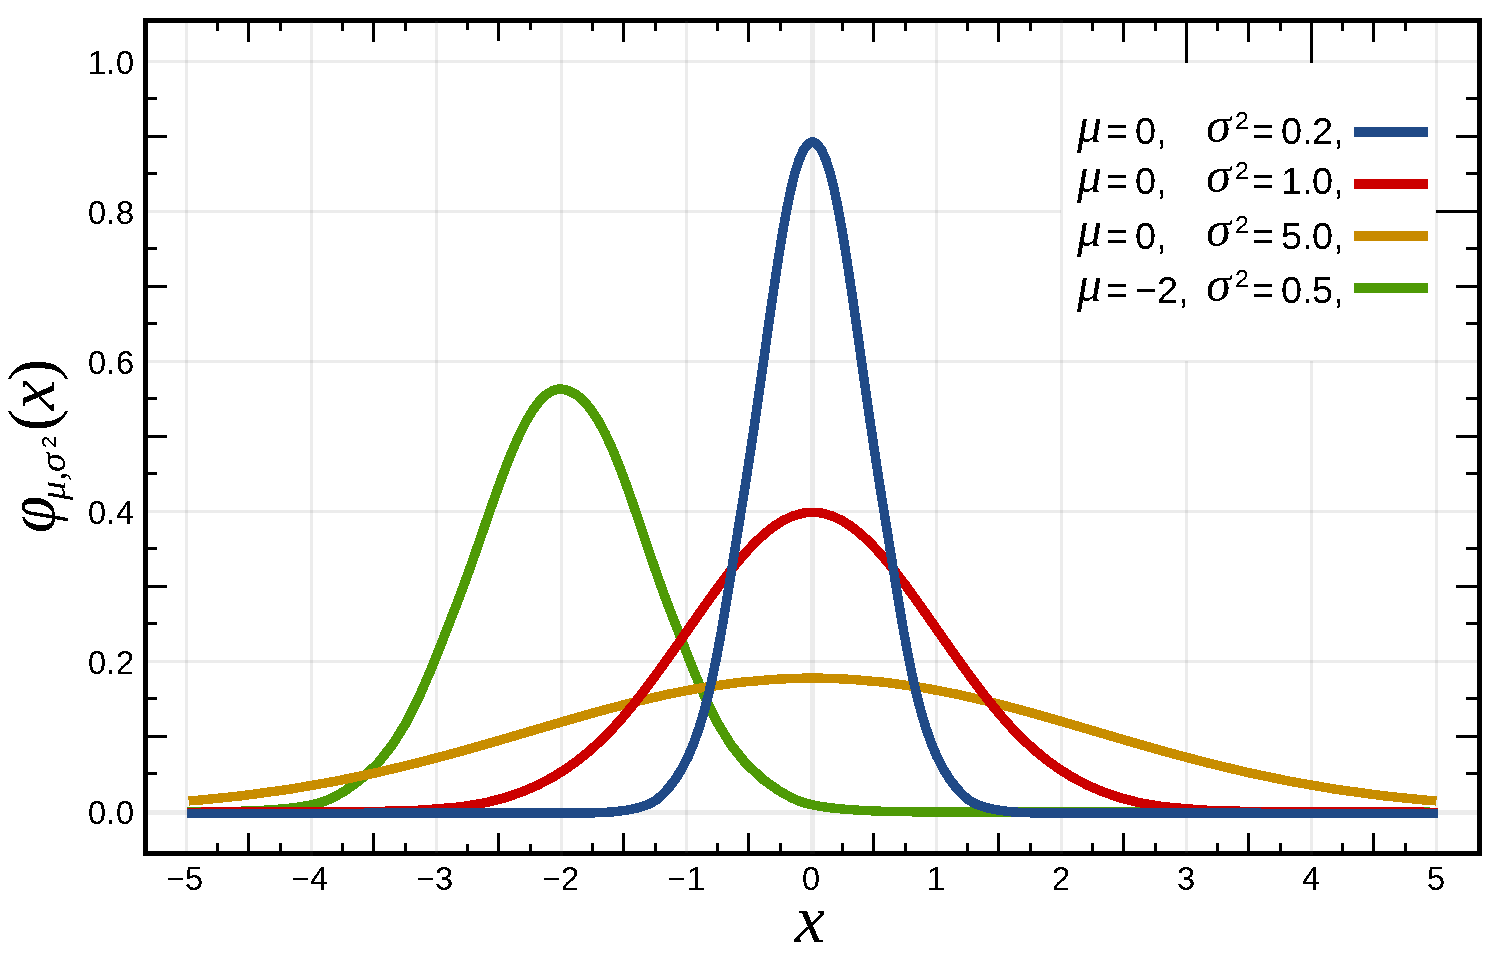
\includegraphics[width=\textwidth]{figures/stats/dist/gaussian_pdf}}
  \caption{Gaussian Distribution PDF}
  \label{fig:dist:gaus}
  \end{subfigure}
  ~
  \begin{subfigure}[b]{\wd\largestimage}\centering
    \usebox{\largestimage}
  \caption{Student's $t$-Distribution PDF}
  \label{fig:dist:student_t}
  \end{subfigure}
\caption{
Gaussian and Student's \tdist PDFs,
by \href{https://en.wikipedia.org/wiki/File:Normal_Distribution_PDF.svg}{Inductiveload}
and \href{https://en.wikipedia.org/wiki/File:Student_t_pdf.svg}{Skbkekas}.
Note that in the limit $\nu \to \infty$ Student's \tdist
approaches the standard normal distribution shown in red.
\label{fig:dist:gaus_student_t}
}
\end{figure}

\begin{figure}
\centering
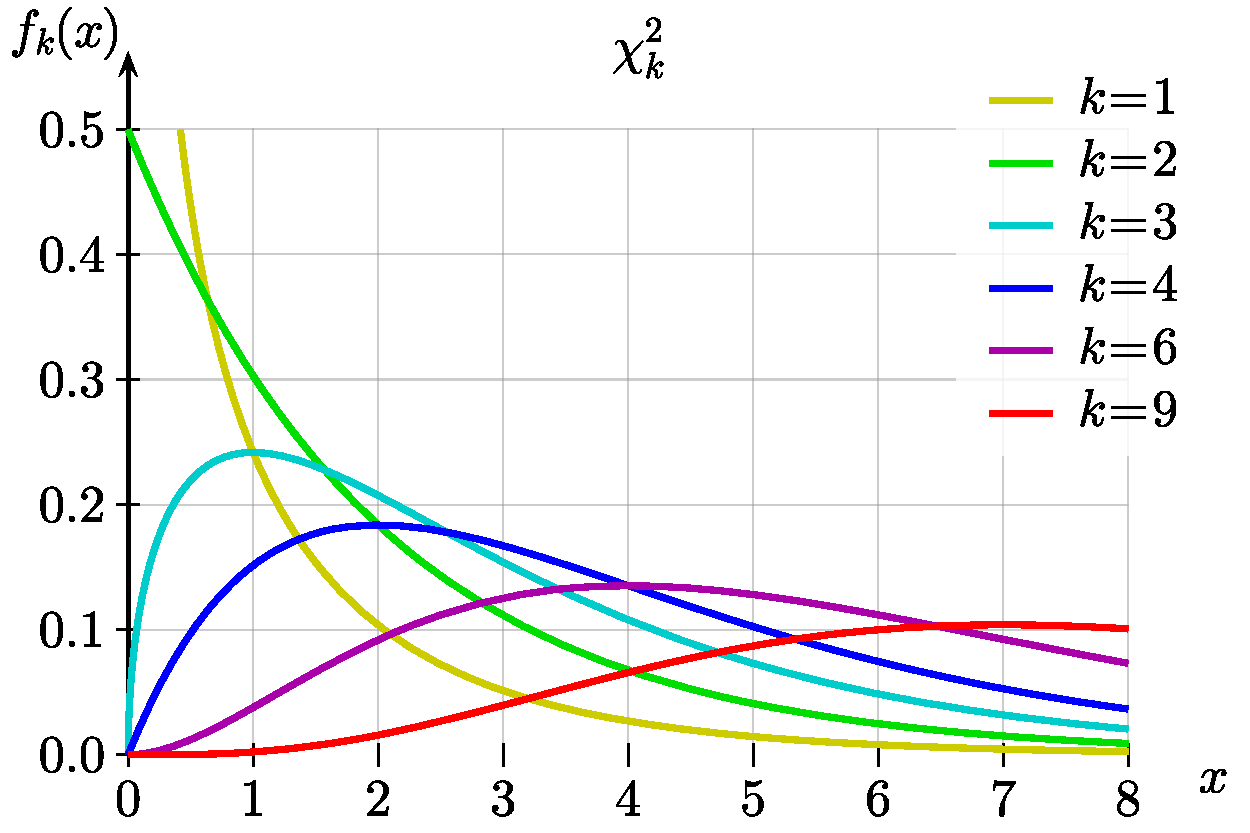
\includegraphics[width=0.7\textwidth]{figures/stats/dist/chi2_pdf}
\caption{
\chiSqdist PDF,
by \href{https://en.wikipedia.org/wiki/File:Chi-square_pdf.svg}{Geek3}.
Here $k$ is being used in lieu of $\nu$ for the number of degrees of freedom.
}
\label{fig:dist:chi2}
\end{figure}

\begin{figure}
\centering
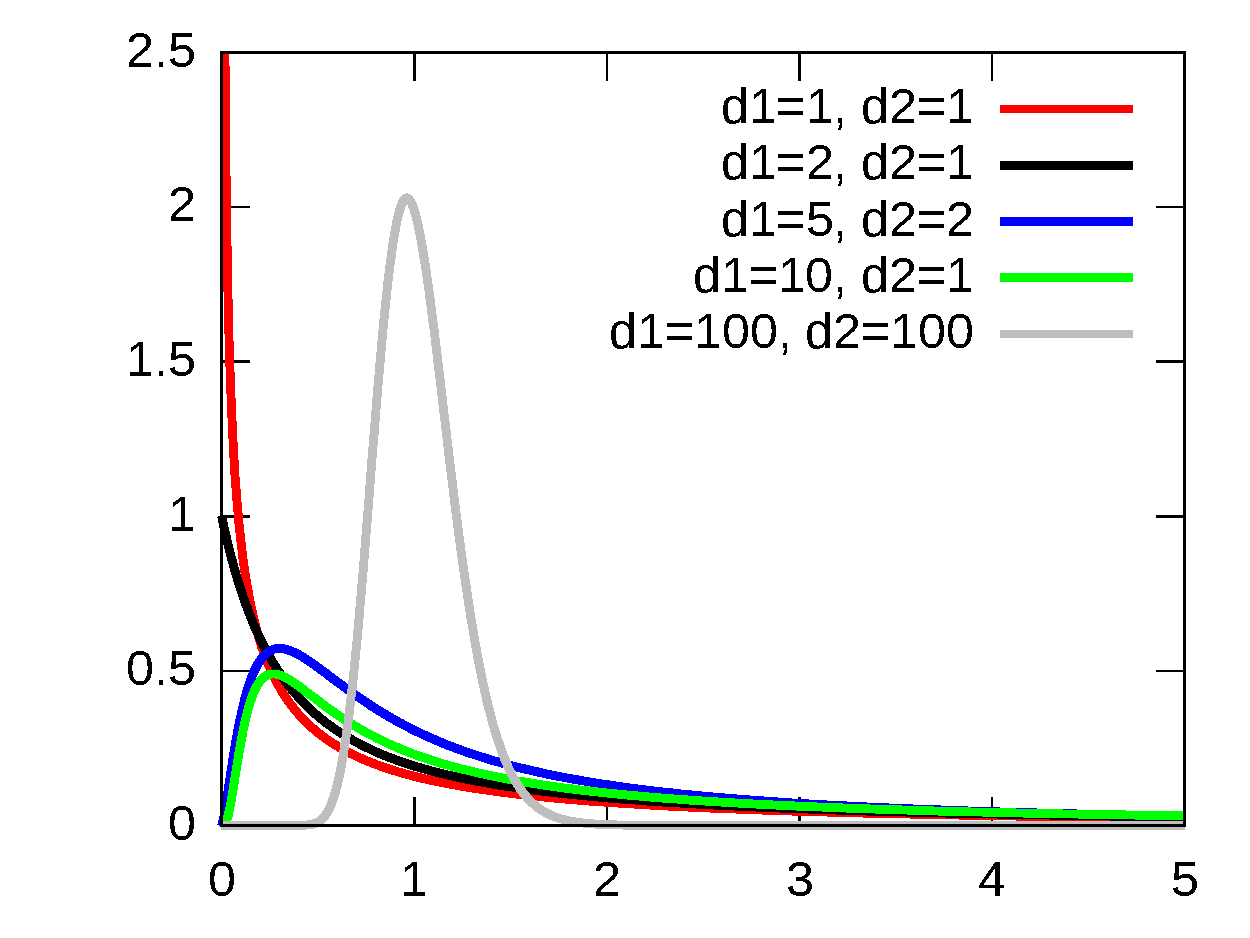
\includegraphics[width=0.7\textwidth,trim={1.5cm 0.1cm 0.1cm 0.1cm},clip]{figures/stats/dist/F_pdf}% trim={<left> <lower> <right> <upper>}
\caption{
\Fdist PDF,
by \href{https://en.wikipedia.org/wiki/File:F-distribution_pdf.svg}{IkamusumeFan}.
}
\label{fig:dist:F}
\end{figure}
